\chapter{Putting LLG Equation in SPICE}

An important step in numerically solving the LLG equation in Cartesian coordinates is the normalization of the magnetization vector to 1 at every step, even in the intermediate steps of the Runge-Kutta algorithm. SPICE can only solve the LLG equation in Cartesian coordinates without the vector normalization step. However, the vector normalization step may be skipped if the LLG equation is solved in the spherical coordinate system instead. In other words: \begin{IEEEeqnarray}{C}
\frac{\partial\bm{m}}{\partial t} = \left(\frac{\partial m_\textit{x}}{\partial t}, \frac{\partial m_\textit{y}}{\partial t}, \frac{\partial m_\textit{z}}{\partial t}\right) \rightarrow \left(\frac{\partial m_\textit{r}}{\partial t}, \frac{\partial m_{\theta}}{\partial t}, \frac{\partial m_{\phi}}{\partial t}\right) = \left(0, \frac{\partial m_{\theta}}{\partial t}, \frac{\partial m_{\phi}}{\partial t}\right)
\end{IEEEeqnarray}The LLG equation consists of three coupled equations in Cartesian coordinates, but only two in spherical coordinates. The LLG equation including the Slonczewski spin-transfer torque term may be written as:\begin{IEEEeqnarray}{rCl}
\frac{\partial\bm{m}}{\partial t} & = & -|\gamma|~\bm{m}\times\bm{H}_\text{EFF} + \alpha~\bm{m}\times\frac{\partial\bm{m}}{\partial t} + \beta_{1}~\bm{m}\times\bm{m}_\textit{p}\times\bm{m} + \beta_{2}~\bm{m}_\textit{p}\times\bm{m} \\
& = & -|\gamma|~\bm{m}\times\left(\bm{H}_\text{EFF} + \frac{\beta_{1}}{|\gamma|}~\bm{m}\times\bm{m}_\textit{p} + \frac{\beta_{2}}{|\gamma|}~\bm{m}_\textit{p}\right) + \alpha~\bm{m}\times\frac{\partial\bm{m}}{\partial t} \label{eq:LLG_implicit}
\end{IEEEeqnarray}where $\bm{H}_\text{EFF}$ is the effective magnetic field experienced by the ferromagnetic domain whose magnetization vector is $\bm{m}$. The terms with $\beta_{1}$ and $\beta_{2}$ are the Slonczewski-like and field-like spin-transfer torque terms, respectively. $\alpha$ is Gilbert's damping factor and $\bm{m}_\textit{p}$ is the spin polarization of the spin current being injected into the ferromagnetic domain. To continue with the derivation, do a self-substitution:\begin{IEEEeqnarray}{rCl}
\frac{\partial\bm{m}}{\partial t} & = & \begin{IEEEeqnarraybox}[][t]{l}
-|\gamma|~\bm{m}\times\left(\bm{H}_\text{EFF} + \frac{\beta_{1}}{|\gamma|}~\bm{m}\times\bm{m}_\textit{p} + \frac{\beta_{2}}{|\gamma|}~\bm{m}_\textit{p}\right) \\
+ \alpha~\bm{m}\times\left(-|\gamma|~\bm{m}\times\left(\bm{H}_\text{EFF} + \frac{\beta_{1}}{|\gamma|}~\bm{m}\times\bm{m}_\textit{p} + \frac{\beta_{2}}{|\gamma|}~\bm{m}_\textit{p}\right) + \alpha~\bm{m}\times\frac{\partial\bm{m}}{\partial t}\right)
\end{IEEEeqnarraybox} \\
\frac{\partial\bm{m}}{\partial t} & = & \begin{IEEEeqnarraybox}[][t]{l}
-|\gamma|~\bm{m}\times\left(\bm{H}_\text{EFF} + \frac{\beta_{1}}{|\gamma|}~\bm{m}\times\bm{m}_\textit{p} + \frac{\beta_{2}}{|\gamma|}~\bm{m}_\textit{p}\right) \\
- \alpha|\gamma|~\bm{m}\times\bm{m}\times\left(\bm{H}_\text{EFF} + \frac{\beta_{1}}{|\gamma|}~\bm{m}\times\bm{m}_\textit{p} + \frac{\beta_{2}}{|\gamma|}~\bm{m}_\textit{p}\right) \\
+ \alpha^{2}~\bm{m}\times\bm{m}\times\frac{\partial\bm{m}}{\partial t}
\end{IEEEeqnarraybox} \label{eq:LLG_implicit_intermediate}
\end{IEEEeqnarray}Next, we note that $\bm{m}$ and $\frac{\partial\bm{m}}{\partial t}$ are orthogonal, which allows us to write Eq.~(\ref{eq:LLG_implicit_intermediate}) as:\begin{IEEEeqnarray}{rCl}
\frac{\partial\bm{m}}{\partial t} & = & \begin{IEEEeqnarraybox}[][t]{l}
-|\gamma|~\bm{m}\times\left(\bm{H}_\text{EFF} + \frac{\beta_{1}}{|\gamma|}~\bm{m}\times\bm{m}_\textit{p} + \frac{\beta_{2}}{|\gamma|}~\bm{m}_\textit{p}\right) \\
- \alpha|\gamma|~\bm{m}\times\bm{m}\times\left(\bm{H}_\text{EFF} + \frac{\beta_{1}}{|\gamma|}~\bm{m}\times\bm{m}_\textit{p} + \frac{\beta_{2}}{|\gamma|}~\bm{m}_\textit{p}\right) \\
- \alpha^{2}~\frac{\partial\bm{m}}{\partial t}
\end{IEEEeqnarraybox} \\
\frac{1+\alpha^{2}}{|\gamma|}\frac{\partial\bm{m}}{\partial t} & = & \begin{IEEEeqnarraybox}[][t]{l}
-\bm{m}\times\left(\bm{H}_\text{EFF} + \frac{\beta_{1}}{|\gamma|}~\bm{m}\times\bm{m}_\textit{p} + \frac{\beta_{2}}{|\gamma|}~\bm{m}_\textit{p}\right) \\
- \alpha~\bm{m}\times\bm{m}\times\left(\bm{H}_\text{EFF} + \frac{\beta_{1}}{|\gamma|}~\bm{m}\times\bm{m}_\textit{p} + \frac{\beta_{2}}{|\gamma|}~\bm{m}_\textit{p}\right)
\end{IEEEeqnarraybox} \label{eq:LLG_explicit}
\end{IEEEeqnarray}Eq.~(\ref{eq:LLG_explicit}) may be rearranged as follows:\begin{IEEEeqnarray}{rCl}
\frac{1+\alpha^{2}}{|\gamma|}\frac{\partial\bm{m}}{\partial t} & = & \begin{IEEEeqnarraybox}[][t]{l}
-\bm{m}\times\bm{H}_\text{EFF} - \alpha~\bm{m}\times\bm{m}\times\bm{H}_\text{EFF} \\
-\frac{\beta_{1}}{|\gamma|}~\bm{m}\times\bm{m}\times\bm{m}_\textit{p} - \frac{\beta_{2}}{|\gamma|}~\bm{m}\times\bm{m}_\textit{p} \\
- \alpha\frac{\beta_{1}}{|\gamma|}~\bm{m}\times\bm{m}\times\bm{m}\times\bm{m}_\textit{p} - \alpha\frac{\beta_{2}}{|\gamma|}~\bm{m}\times\bm{m}\times\bm{m}_\textit{p}
\end{IEEEeqnarraybox} \\
& = & \begin{IEEEeqnarraybox}[][t]{l}
-\bm{m}\times\bm{H}_\text{EFF} - \alpha~\bm{m}\times\bm{m}\times\bm{H}_\text{EFF} \\
-\frac{\beta_{1}+\alpha\beta_{2}}{|\gamma|}~\bm{m}\times\bm{m}\times\bm{m}_\textit{p} \\
- \frac{\beta_{2}}{|\gamma|}~\bm{m}\times\bm{m}_\textit{p} - \alpha\frac{\beta_{1}}{|\gamma|}~\bm{m}\times\bm{m}\times\bm{m}\times\bm{m}_\textit{p}
\end{IEEEeqnarraybox} \label{eq:LLG_explicit_cart}
\end{IEEEeqnarray}By noting that:\begin{IEEEeqnarray}{rCl}
\bm{m}\times\bm{m}\times\bm{m}\times\bm{m}_\textit{p} & = & -\bm{m}\times\bm{m}_\textit{p} \label{eq:tripcross}
\end{IEEEeqnarray}Substituting Eq.~(\ref{eq:tripcross}) into Eq.~(\ref{eq:LLG_explicit_cart}), we arrive at:\begin{IEEEeqnarray}{rCl}
\frac{1+\alpha^{2}}{|\gamma|}\frac{\partial\bm{m}}{\partial t} & = & \begin{IEEEeqnarraybox}[][t]{l}
-\bm{m}\times\bm{H}_\text{EFF} - \alpha~\bm{m}\times\bm{m}\times\bm{H}_\text{EFF} \\
-\frac{\beta_{1}+\alpha\beta_{2}}{|\gamma|}~\bm{m}\times\bm{m}\times\bm{m}_\textit{p} - \frac{\beta_{2}-\alpha\beta_{1}}{|\gamma|}~\bm{m}\times\bm{m}_\textit{p}
\end{IEEEeqnarraybox} \label{eq:LLGS_Cart}
\end{IEEEeqnarray}Thus, the cross-product terms need to be expressed in spherical coordinates.

In converting from Cartesian to spherical coordinate system, we need to derive the basis vector for spherical coordinate system. We may then resolve $\frac{\partial\bm{m}}{\partial t}$ everywhere in 3-dimension space. Starting with:\begin{IEEEeqnarray}{rCl}
\bm{r} & = & \left(\begin{IEEEeqnarraybox}[][c]{C}
\text{sin}~\theta~\text{cos}~\phi \\
\text{sin}~\theta~\text{sin}~\phi \\
\text{cos}~\theta \end{IEEEeqnarraybox}\right) \\
\bm{z} & = & \left(\begin{IEEEeqnarraybox}[][c]{C}
0 \\
0 \\
1 \end{IEEEeqnarraybox}\right) \\
\bm{\phi} & = & \frac{\bm{z}\times\bm{r}}{|\bm{z}\times\bm{r}|} =\frac{1}{\text{sin}~\theta} \left(\begin{IEEEeqnarraybox}[][c]{C}
0 \\
0 \\
1 \end{IEEEeqnarraybox}\right)\times\left(\begin{IEEEeqnarraybox}[][c]{C}
\text{sin}~\theta~\text{cos}~\phi \\
\text{sin}~\theta~\text{sin}~\phi \\
\text{cos}~\theta \end{IEEEeqnarraybox}\right) = \frac{1}{\text{sin}~\theta}\left(\begin{IEEEeqnarraybox}[][c]{C}
-\text{sin}~\theta~\text{sin}~\phi \\
\text{sin}~\theta~\text{cos}~\phi \\
0 \end{IEEEeqnarraybox}\right) \\
& = & \left(\begin{IEEEeqnarraybox}[][c]{C}
-\text{sin}~\phi \\
\text{cos}~\phi \\
0 \end{IEEEeqnarraybox}\right) \\
\bm{\theta} & = & \bm{\phi}\times\bm{r} = \left(\begin{IEEEeqnarraybox}[][c]{C}
-\text{sin}~\phi \\
\text{cos}~\phi \\
0 \end{IEEEeqnarraybox}\right)\times\left(\begin{IEEEeqnarraybox}[][c]{C}
\text{sin}~\theta~\text{cos}~\phi \\
\text{sin}~\theta~\text{sin}~\phi \\
\text{cos}~\theta \end{IEEEeqnarraybox}\right) = \left(\begin{IEEEeqnarraybox}[][c]{C}
\text{cos}~\theta~\text{cos}~\phi \\
\text{cos}~\theta~\text{sin}~\phi \\
-\text{sin}~\theta \end{IEEEeqnarraybox}\right)
\end{IEEEeqnarray}In summary, the basis vectors we want are:\begin{IEEEeqnarray}{rClrClrCl}
\bm{r} & = & \left(\begin{IEEEeqnarraybox}[][c]{C}
\text{sin}~\theta~\text{cos}~\phi \\
\text{sin}~\theta~\text{sin}~\phi \\
\text{cos}~\theta \end{IEEEeqnarraybox}\right) & ,~\bm{\phi} & = & \left(\begin{IEEEeqnarraybox}[][c]{C}
-\text{sin}~\phi \\
\text{cos}~\phi \\
0 \end{IEEEeqnarraybox}\right) & ,~\bm{\theta} & = & \left(\begin{IEEEeqnarraybox}[][c]{C}
\text{cos}~\theta~\text{cos}~\phi \\
\text{cos}~\theta~\text{sin}~\phi \\
-\text{sin}~\theta \end{IEEEeqnarraybox}\right)
\end{IEEEeqnarray}

Next, the cross-products may be written as:\begin{IEEEeqnarray}{rCl}
\bm{a}\times\bm{b} & = & \left(\begin{IEEEeqnarraybox}[][c]{C}
a_\textit{x} \\
a_\textit{y} \\
a_\textit{z} \end{IEEEeqnarraybox}\right)\times\left(\begin{IEEEeqnarraybox}[][c]{C}
b_\textit{x} \\
b_\textit{y} \\
b_\textit{z} \end{IEEEeqnarraybox}\right) = \left(\begin{IEEEeqnarraybox}[][c]{C}
a_\textit{y}b_\textit{z} - a_\textit{z}b_\textit{y} \\
a_\textit{z}b_\textit{x} - a_\textit{x}b_\textit{z} \\
a_\textit{x}b_\textit{y} - a_\textit{y}b_\textit{x} \end{IEEEeqnarraybox}\right) \\
\bm{a}\times\bm{a}\times\bm{b} & = & \left(\begin{IEEEeqnarraybox}[][c]{C}
a_\textit{x} \\
a_\textit{y} \\
a_\textit{z} \end{IEEEeqnarraybox}\right)\times\left(\begin{IEEEeqnarraybox}[][c]{C}
a_\textit{y}b_\textit{z} - a_\textit{z}b_\textit{y} \\
a_\textit{z}b_\textit{x} - a_\textit{x}b_\textit{z} \\
a_\textit{x}b_\textit{y} - a_\textit{y}b_\textit{x} \end{IEEEeqnarraybox}\right) = \left(\begin{IEEEeqnarraybox}[][c]{C}
(a_\textit{x}b_\textit{x} + a_\textit{y}b_\textit{y} + a_\textit{z}b_\textit{z})a_\textit{x} \\
(a_\textit{x}b_\textit{x} + a_\textit{y}b_\textit{y} + a_\textit{z}b_\textit{z})a_\textit{y} \\
(a_\textit{x}b_\textit{x} + a_\textit{y}b_\textit{y} + a_\textit{z}b_\textit{z})a_\textit{z} \end{IEEEeqnarraybox}\right) - \left(\begin{IEEEeqnarraybox}[][c]{C}
(a^{2}_\textit{x}+a^{2}_\textit{y}+a^{2}_\textit{z})b_\textit{x} \\
(a^{2}_\textit{x}+a^{2}_\textit{y}+a^{2}_\textit{z})b_\textit{y} \\
(a^{2}_\textit{x}+a^{2}_\textit{y}+a^{2}_\textit{z})b_\textit{z} \end{IEEEeqnarraybox}\right) \\
& = & (\bm{a}\cdot\bm{b})\bm{a} - |\bm{a}|^{2}\bm{b}
\end{IEEEeqnarray}

Let us now perform the cross-product conversion noting that $\bm{m}=\bm{r}$. Then, for any general vector, $\bm{a}$:\begin{IEEEeqnarray}{rCl}
(\bm{r}\times\bm{a})_{\phi} & = & (\bm{r}\times\bm{a})\cdot\bm{\phi} \label{eq:cross_top} \\
& = & (-\text{sin}~\phi)(a_\textit{z}\text{sin}~\theta~\text{sin}~\phi - a_\textit{y}\text{cos}~\theta) + (\text{cos}~\phi)(a_\textit{x}\text{cos}~\theta- a_\textit{z}~\text{sin}~\theta~\text{cos}~\phi) \\
& = & a_\textit{x}\text{cos}~\theta~\text{cos}~\phi + a_\textit{y}~\text{cos}~\theta~\text{sin}~\phi - a_\textit{z}\text{sin}~\theta \\
& = & \bm{a}\cdot\bm{\theta} \\
(\bm{r}\times\bm{a})_{\theta} & = & (\bm{r}\times\bm{a})\cdot\bm{\theta} \\
& = & \begin{IEEEeqnarraybox}[][t]{l}
(\text{cos}~\theta~\text{cos}~\phi)(a_\textit{z}\text{sin}~\theta~\text{sin}~\phi - a_\textit{y}\text{cos}~\theta) + (\text{cos}~\theta~\text{sin}~\phi)(a_\textit{x}\text{cos}~\theta - a_\textit{z}\text{sin}~\theta~\text{cos}~\phi) \\
- (\text{sin}~\theta)(a_\textit{y}\text{sin}~\theta~\text{cos}~\phi - a_\textit{x}\text{sin}~\theta~\text{sin}~\phi)
\end{IEEEeqnarraybox} \\
& = & a_\textit{x}\text{sin}~\phi - a_\textit{y}\text{cos}~\phi \\
& = & -\bm{a}\cdot\bm{\phi}
\end{IEEEeqnarray}and for the double cross-products:\begin{IEEEeqnarray}{rCl}
(\bm{r}\times\bm{r}\times\bm{a})_{\phi} & = & (\bm{r}\times\bm{r}\times\bm{a})\cdot\bm{\phi} = ((\bm{r}\cdot\bm{a})\bm{r} - |\bm{r}|^{2}\bm{a})\cdot\bm{\phi} = (\bm{r}\cdot\bm{a})\bm{r}\cdot\bm{\phi} -  |\bm{r}|^{2}\bm{a}\cdot\bm{\phi} = -\bm{a}\cdot\bm{\phi} \\
(\bm{r}\times\bm{r}\times\bm{a})_{\theta} & = & (\bm{r}\times\bm{r}\times\bm{a})\cdot\bm{\theta} = ((\bm{r}\cdot\bm{a})\bm{r} - |\bm{r}|^{2}\bm{a})\cdot\bm{\theta} = (\bm{r}\cdot\bm{a})\bm{r}\cdot\bm{\theta} -  |\bm{r}|^{2}\bm{a}\cdot\bm{\theta} = -\bm{a}\cdot\bm{\theta} \label{eq:cross_bot}
\end{IEEEeqnarray}Now, we write Eq.~(\ref{eq:LLGS_Cart}) in spherical coordinates using Eqs.~(\ref{eq:cross_top})--(\ref{eq:cross_bot}):\begin{IEEEeqnarray}{rCl}
\frac{1+\alpha^{2}}{|\gamma|}\frac{\partial{}m_{\theta}}{\partial t} & = & \bm{H}_\text{EFF}\cdot(\bm{\phi}+\alpha\bm{\theta}) + \frac{\beta_{1}}{|\gamma|}\bm{m}_\textit{p}\cdot(\bm{\theta}-\alpha\bm{\phi}) + \frac{\beta_{2}}{|\gamma|}\bm{m}_\textit{p}\cdot(\bm{\phi}+\alpha\bm{\theta}) \label{eq:SPICE_LLG_top} \\
& = & \left(\alpha\bm{H}_\text{EFF}+\frac{\beta_{1}+\alpha\beta_{2}}{|\gamma|}\bm{m}_\textit{p}\right)\cdot\bm{\theta} + \left(\bm{H}_\text{EFF}+\frac{\beta_{2}-\alpha\beta_{1}}{|\gamma|}\bm{m}_\textit{p}\right)\cdot\bm{\phi} \\
\frac{1+\alpha^{2}}{|\gamma|}\frac{\partial{}m_{\phi}}{\partial t} & = & \bm{H}_\text{EFF}\cdot(\alpha\bm{\phi}-\bm{\theta}) + \frac{\beta_{1}}{|\gamma|}\bm{m}_\textit{p}\cdot(\bm{\phi}+\alpha\bm{\theta}) + \frac{\beta_{2}}{|\gamma|}\bm{m}_\textit{p}\cdot(\alpha\bm{\phi}-\bm{\theta}) \\
& = & \left(\alpha\bm{H}_\text{EFF}+\frac{\beta_{1}+\alpha\beta_{2}}{|\gamma|}\bm{m}_\textit{p}\right)\cdot\bm{\phi} - \left(\bm{H}_\text{EFF} + \frac{\beta_{2}-\alpha\beta_{1}}{|\gamma|}\bm{m}_\textit{p}\right)\cdot\bm{\theta} \label{eq:SPICE_LLG_bot}
\end{IEEEeqnarray}Eqs.~(\ref{eq:SPICE_LLG_top})--(\ref{eq:SPICE_LLG_bot}) are sufficient for generating a SPICE subcircuit that solves the LLG equation.\begin{figure}[b]
\centering
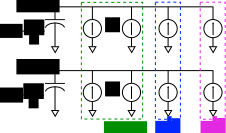
\includegraphics[scale=1.25]{LLG4SPICE/figs/SPICE_LLG_Circuit}
\caption{The schematic of a subcircuit that is used to enable SPICE to solve the LLG equation. Scalar multipliers for each current source are left out for clarity.}
\label{fig:model_schematic}
\end{figure}

Each term on the left-hand side of Eqs.~(\ref{eq:SPICE_LLG_top})--(\ref{eq:SPICE_LLG_bot}) is represented as the voltage across a capacitor as shown in Fig.~\ref{fig:model_schematic}. Each term on the right-hand side of Eqs.~(\ref{eq:SPICE_LLG_top})--(\ref{eq:SPICE_LLG_bot}) is represented as a current source with positive direction of current flow as indicated in Fig.~\ref{fig:model_schematic}. $\bm{H}_\text{EFF}$ is a linear combination of magnetic fields:\begin{IEEEeqnarray}{rCl}
\bm{H}_\text{EFF} & = & \sum_{i}\bm{H}_{i}
\end{IEEEeqnarray}The current sources to represent a generic magnetic field, $\bm{H} = (H_\textit{x}, H_\textit{y}, H_\textit{z})$, $\theta = \textit{V}_\textit{C1}$ and $\phi = \textit{V}_\textit{C2}$, are:\begin{IEEEeqnarray}{l}
\text{For~driving~into~}m_{\theta}:~H_\textit{x}(-\text{sin}~\phi + \alpha~\text{cos}~\theta~\text{cos}~\phi) + H_\textit{y}(\text{cos}~\phi + \alpha~\text{cos}~\theta~\text{sin}~\phi) + H_\textit{z}(-\alpha~\text{sin}~\theta) \\
\text{For~driving~into~}m_{\phi}:~H_\textit{x}(-\alpha~\text{sin}~\phi - \text{cos}~\theta~\text{cos}~\phi) + H_\textit{y}(\alpha~\text{cos}~\phi - \text{cos}~\theta~\text{sin}~\phi) + H_\textit{z}(\text{sin}~\theta)
\end{IEEEeqnarray}

The anisotropy fields can be modeled by considering $\bm{H}_\text{anisotropy} = -\bm{N}\bm{m}$, where:\begin{IEEEeqnarray}{rCl}
\bm{N} & = & M_\text{sat}\left(\begin{IEEEeqnarraybox}[][c]{CCC}
N_\textit{xx} & 0 & 0 \\
0 & N_\textit{yy} & 0 \\
0 & 0 & N_\textit{zz}
\end{IEEEeqnarraybox} \right)
\end{IEEEeqnarray}Consider easy-plane anisotropy, where the plane of the ferromagnet is in the \textit{xy}-plane. Then, \begin{IEEEeqnarray}{C}
N_\textit{xx} = 0,~N_\textit{yy} = 0,~N_\textit{zz} = -4\pi{}M_\text{sat}
\end{IEEEeqnarray}and the current sources to represent the easy-plane anisotropy field are given by:\begin{IEEEeqnarray}{l}
\text{For~driving~into~}m_{\theta}:~2\pi\alpha{}M_\text{sat}~\text{sin}(2\theta) \\
\text{For~driving~into~}m_{\phi}:~-2\pi{}M_\text{sat}\text{sin}(2\theta)
\end{IEEEeqnarray}For uniaxial anisotropy in which the easy-axis is along the \textit{x}-axis:\begin{IEEEeqnarray}{C}
N_\textit{xx} = \frac{2K_\textit{u2}}{\mu_{0}M^{2}_\text{sat}},~N_\textit{yy} = 0,~N_\textit{zz} = 0
\end{IEEEeqnarray}and the current sources to represent the easy-plane anisotropy field are given by:\begin{IEEEeqnarray}{l}
\text{For~driving~into~}m_{\theta}:~\frac{2K_\textit{u2}}{\mu_{0}M_\text{sat}}\text{sin}~\theta~\text{cos}~\phi~(\text{cos}~\phi + \alpha~\text{cos}~\theta~\text{cos}~\phi) \\
\text{For~driving~into~}m_{\phi}:~\frac{2K_\textit{u2}}{\mu_{0}M_\text{sat}}\text{sin}~\theta~\text{cos}~\phi~(\text{cos}~\phi + \alpha~\text{cos}~\theta~\text{cos}~\phi)
\end{IEEEeqnarray}For uniaxial anisotropy in which the easy-axis is along the \textit{y}-axis:\begin{IEEEeqnarray}{C}
N_\textit{xx} = 0,~N_\textit{yy} = \frac{2K_\textit{u2}}{\mu_{0}M^{2}_\text{sat}},~N_\textit{zz} = 0
\end{IEEEeqnarray}and the current sources to represent the easy-plane anisotropy field are given by:\begin{IEEEeqnarray}{l}
\text{For~driving~into~}m_{\theta}:~\frac{2K_\textit{u2}}{M_\text{sat}}\text{sin}~\theta~\text{sin}~\phi~(-\text{sin}~\phi + \alpha~\text{cos}~\theta~\text{sin}~\phi) \\
\text{For~driving~into~}m_{\phi}:~\frac{2K_\textit{u2}}{\mu_{0}M_\text{sat}}\text{sin}~\theta~\text{sin}~\phi~(-\alpha~\text{sin}~\phi - \text{cos}~\theta~\text{sin}~\phi)
\end{IEEEeqnarray}For uniaxial anisotropy in which the easy-axis is along the \textit{z}-axis:\begin{IEEEeqnarray}{C}
N_\textit{xx} = 0,~N_\textit{yy} = 0,~N_\textit{zz} = \frac{2K_\textit{u2}}{\mu_{0}M^{2}_\text{sat}}
\end{IEEEeqnarray}and the current sources to represent the easy-plane anisotropy field are given by:\begin{IEEEeqnarray}{l}
\text{For~driving~into~}m_{\theta}:~-\frac{\alpha{}K_\textit{u2}}{M_\text{sat}}~\text{sin}(2\theta) \\
\text{For~driving~into~}m_{\phi}:~\frac{K_\textit{u2}}{M_\text{sat}}~\text{sin}(2\theta)
\end{IEEEeqnarray}

For the spin-transfer torque terms, we have:\begin{IEEEeqnarray}{C}
\begin{IEEEeqnarraybox}[][c]{rClrCl}
\beta_{1} & = & |\gamma|\beta\epsilon & ,~\beta_{2} & = & |\gamma|\beta\epsilon\text{'}
\end{IEEEeqnarraybox} \label{eq:betas} \\
\begin{IEEEeqnarraybox}[][c]{rCl}
\beta & = & \left|\frac{\hbar}{\mu_{0}e}\right|\frac{J}{tM_\text{sat}}
\end{IEEEeqnarraybox}
\end{IEEEeqnarray}where $t$ is the dimension of the ferromagnet along the direction of current flow. Hence, the factors in Eqs.~(\ref{eq:SPICE_LLG_top})--(\ref{eq:SPICE_LLG_bot}) reduce to:\begin{IEEEeqnarray}{C}
\begin{IEEEeqnarraybox}[][c]{rClrCl}
\frac{\beta_{1}+\alpha\beta_{2}}{|\gamma|} & = & \beta(\epsilon+\alpha\epsilon\text{'}) =  \left|\frac{\hbar}{\mu_{0}e}\right|\frac{J}{tM_\text{sat}}(\epsilon+\alpha\epsilon\text{'}) & ;~\frac{\beta_{2}-\alpha\beta_{1}}{|\gamma|} & = & \beta(\epsilon\text{'} - \alpha\epsilon) = \left|\frac{\hbar}{\mu_{0}e}\right|\frac{J}{tM_\text{sat}}(\epsilon\text{'} - \alpha\epsilon)
\end{IEEEeqnarraybox} \label{eq:betas_simpliied}
\end{IEEEeqnarray}In a micromagnetic solver like the Object-Oriented MicroMagnetic Framework (OOMMF), $\epsilon\text{'}$ is a constant parameter and:\begin{IEEEeqnarray}{rCl}
\epsilon & = & \frac{q_{+}}{A_{+}+A_{-}(\bm{m}\cdot\bm{m}_\textit{p})} + \frac{q_{-}}{A_{+}-A_{-}(\bm{m}\cdot\bm{m}_\textit{p})} \\
A_{\pm} & = & \sqrt{(\Lambda^{2}_\textit{PL}\pm{}1)(\Lambda^{2}_\textit{FL}\pm{}1)} \\
q_{\pm} & = & \textit{P}_\textit{PL}\Lambda^{2}_\textit{PL}\sqrt{\frac{\Lambda^{2}_\textit{FL}+1}{\Lambda^{2}_\textit{PL}+1}} \pm \textit{P}_\textit{FL}\Lambda^{2}_\textit{FL}\sqrt{\frac{\Lambda^{2}_\textit{PL}-1}{\Lambda^{2}_\textit{FL}-1}}
\end{IEEEeqnarray}where $\textit{P}_\textit{FL}$ and $\textit{P}_\textit{PL}$ are the polarization factors of the free layer and pinned layer, respectively, and $\Lambda_\textit{FL}$ and $\Lambda_\textit{PL}$ are related to the density of states around the Fermi energy in the free layer and pinned layer, respectively.

It can be clearly seen in Eqs.~(\ref{eq:SPICE_LLG_top})--(\ref{eq:SPICE_LLG_bot}) that the spin-torque term containing $\beta_{2}$ has the same form as a magnetic field (hence it is called the ``field-like term''). The current sources to represent the field-like term are:\begin{IEEEeqnarray}{rl}
\text{For~driving~into~}m_{\theta}:~ & \begin{IEEEeqnarraybox}[][t]{l}
\left|\frac{\hbar}{\mu_{0}e}\right|\frac{J}{tM_\text{sat}}\epsilon\text{'}[m_\textit{p,x}(-\text{sin}~\phi + \alpha~\text{cos}~\theta~\text{cos}~\phi) + m_\textit{p,y}(\text{cos}~\phi + \alpha~\text{cos}~\theta~\text{sin}~\phi) \\
+ m_\textit{p,z}(-\alpha~\text{sin}~\theta)]
\end{IEEEeqnarraybox} \\
\text{For~driving~into~}m_{\phi}:~ & \begin{IEEEeqnarraybox}[][t]{l}
\left|\frac{\hbar}{\mu_{0}e}\right|\frac{J}{tM_\text{sat}}\epsilon\text{'}[m_\textit{p,x}(-\alpha~\text{sin}~\phi - \text{cos}~\theta~\text{cos}~\phi) + m_\textit{p,y}(\alpha~\text{cos}~\phi - \text{cos}~\theta~\text{sin}~\phi) \\
+ m_\textit{p,z}(\text{sin}~\theta)]
\end{IEEEeqnarraybox}
\end{IEEEeqnarray}The Slonczewski-like spin-torque term are the terms containing $\beta_{1}$ in Eqs.~(\ref{eq:SPICE_LLG_top})--(\ref{eq:SPICE_LLG_bot}), and are represented using the current sources written as:\begin{IEEEeqnarray}{rl}
\text{For~driving~into~}m_{\theta}:~ & \begin{IEEEeqnarraybox}[][t]{l}
\left|\frac{\hbar}{\mu_{0}e}\right|\frac{J}{tM_\text{sat}}\epsilon[m_\textit{p,x}(\alpha~\text{sin}~\phi + \text{cos}~\theta~\text{cos}~\phi) + m_\textit{p,y}(\text{cos}~\theta~\text{sin}~\phi - \alpha~\text{cos}~\phi) \\
+ m_\textit{p,z}(-\text{sin}~\theta)]
\end{IEEEeqnarraybox} \\
\text{For~driving~into~}m_{\phi}:~ & \begin{IEEEeqnarraybox}[][t]{l}
\left|\frac{\hbar}{\mu_{0}e}\right|\frac{J}{tM_\text{sat}}\epsilon[m_\textit{p,x}(-\text{sin}~\phi + \alpha~\text{cos}~\theta~\text{cos}~\phi) + m_\textit{p,y}(\text{cos}~\phi + \alpha~\text{cos}~\theta~\text{sin}~\phi) \\
+ m_\textit{p,z}(- \alpha~\text{sin}~\theta)]
\end{IEEEeqnarraybox}
\end{IEEEeqnarray}